%%!TEX encoding = UTF-8 Unicode

% According to UA rules, font size should range from 10 to 12pt.
\documentclass[11pt,a4paper,openright,twoside,onecolumn]{memoir}

\listfiles
\fixpdflayout

\usepackage[utf8]{inputenc}

% Computer Modern Typewritter (For bold ttfamily in listings)
\usepackage{lmodern}
% OR... Bera Mono
%\usepackage[scaled]{beramono} % TTT Font
%\usepackage{anyfontsize} % As the name says...

\usepackage[T1]{fontenc}

% For Overleaf support
\usepackage{ifthen}
\def\useoverleaf{1}  % change to non-zero (for instance, 1) to enable it

\makeatletter
\newcommand{\makecoverfile}[0]{%
  \immediate\write18{latexmk -pdf cover.tex}%
}
\makeatother

%For PDF merging
\usepackage{pdfpages}

%SET DPI to 300
\pdfpxdimen=\dimexpr 1in/300\relax

\usepackage{morewrites} % Allow the use of a larger number of packages

%For English and Portuguese languages
%Portuguese will be the default.
%Use \setdefaultlanguage to change it

%\usepackage[english,portuguese]{babel}
\usepackage[english]{babel}

% Uncomment to use a custom date format
%\usepackage{datetime}
%\newdateformat{thesisdate}{\monthname[\THEMONTH] \THEYEAR} % Month Year

\usepackage{microtype} % Make pdf look better


% Uncomment to enable floats on facing pages
%\usepackage{dpfloat}

%Side by side figures
% Eg. Fig 1a, Fig 1b
\usepackage[hang,small,bf]{caption}
%\let\tion\undefined
%\let\subfloat\undefined
\usepackage{subcaption}

%\RequirePackage{textcase}

% Dropped Caps
%\usepackage{lettrine}


% Configure Hyperlink color
%\usepackage[breaklinks=true,colorlinks=false,linkcolor=blue]{hyperref}
% Or use the default
\usepackage{hyperref}

%Optional: Redefine section names
%\def\sectionautorefname{Section}
%\def\chapterautorefname{Chapter}
%\def\figureautorefname{Figure}
%\def\listingautorefname{Listing}
%\def\tableautorefname{Table}

%For PDF Comments
\usepackage{comment}
\ifthenelse{\equal{\useoverleaf}{0}}
{\usepackage{pdfcomment}}{}
\usepackage{bookmark} % New Bookmarks

%For Multiple columns in Glossary
\usepackage{multicol}

%Math symbols
\usepackage{amsmath}
\usepackage{amssymb}

%Graphics
\usepackage{graphicx}

%Colors
\usepackage{xcolor}

%Euro symbol
\usepackage{eurosym}

% Code boxes
\ifthenelse{\equal{\useoverleaf}{0}}
{\usepackage[outputdir=build]{minted}}
{\usepackage{minted}}%

\renewcommand\listingscaption{Código}
\fvset{fontsize=\footnotesize} % Make Code blocks smaller than text
\usepackage{csquotes}

%Biber using IEEE style for proper UTF-8 support
\usepackage[backend=biber,style=ieee, sorting=none]{biblatex}
\bibliography{bib/HumanActionPrediction&Anticipation.bib}

%Use acronyms
\usepackage[printonlyused]{acronym} % For acronyms

% For indenting the first paragraph after section start
\usepackage{indentfirst}

% Enable chart support through pgf and tikz
\usepackage[version=0.96]{pgf}
\usepackage{tikz}
\usepackage{pgf-umlsd}
\usetikzlibrary{arrows,shadows,trees,shapes,decorations,automata,backgrounds,petri,mindmap} % for pgf-umlsd

%For Electric Circuits
\usepackage[detect-weight=true, binary-units=true]{siunitx}
\sisetup{load-configurations = binary}

% Set Voltage direction accordingly
% Option : oldvoltagedirection,nooldvoltagedirection,RPvoltages,EFvoltages
% More information at: https://mirrors.ibiblio.org/CTAN/graphics/pgf/contrib/circuitikz/doc/circuitikzmanual.pdf
%By default this template is using the Old Voltage Direction
\usepackage[oldvoltagedirection,american,cuteinductors,smartlabels]{circuitikz}

\usetikzlibrary{calc}
\ctikzset{bipoles/thickness=1}
\ctikzset{bipoles/length=0.8cm}
\ctikzset{bipoles/diode/height=.375}
\ctikzset{bipoles/diode/width=.3}
\ctikzset{tripoles/thyristor/height=.8}
\ctikzset{tripoles/thyristor/width=1}
\ctikzset{bipoles/vsourceam/height/.initial=.7}
\ctikzset{bipoles/vsourceam/width/.initial=.7}
\tikzstyle{every node}=[font=\small]
\tikzstyle{every path}=[line width=0.8pt,line cap=round,line join=round]

% For inline TT text (e.g. code snippets)
\usepackage{verbatim}

 %Frames around figures and allow force placement
\usepackage{float}

%Configure Float style
%\floatstyle{boxed}
%\restylefloat{table}
%\restylefloat{figure}
%\restylefloat{lstlisting}

%For test purposes
\usepackage{lipsum}

%Keep floats inside section!
\usepackage[section]{placeins}
\let \oldsubsubsection \subsubsection
\renewcommand{\subsubsection}[2][]{
  \FloatBarrier
  \oldsubsubsection#1{#2}
}
\let \oldsubsection \subsection
\renewcommand{\subsection}[2][]{
  \FloatBarrier
  \oldsubsection#1{#2}
}
\let \oldsection \section
\renewcommand{\section}[2][]{
  \FloatBarrier
  \oldsection#1{#2}
}
\let \oldchapter \chapter
\renewcommand{\chapter}[2][]{
  \FloatBarrier
  \oldchapter#1{#2}
}


%%%% Use the built-in division styling
\headstyles{memman}

%%% ToC down to subsections
\settocdepth{subsection}

%%% Numbering down to subsections as well
\setsecnumdepth{subsection}

%%%% extra index for first lines
\makeindex[lines]

%Margins for University of Aveiro Thesis
\setlrmarginsandblock{3cm}{2.5cm}{*}
\setulmarginsandblock{3cm}{3cm}{*}
\checkandfixthelayout

%Or custom spacing
%\addtolength{\parskip}{0.5\baselineskip}
\linespread{1.5}

\begin{document}
\ifthenelse{\equal{\useoverleaf}{0}}{}{\makecoverfile{}}%
\includepdf[pages=-]{cover.pdf}

%
%Front matter

%Custom Chapter style named thesis
\makechapterstyle{thesis}{% Based on ell
  \chapterstyle{default}
  \renewcommand*{\chapnumfont}{\normalfont\sffamily}
  \renewcommand*{\chaptitlefont}{\normalfont\Huge\sffamily}
  \settowidth{\chapindent}{\chapnumfont 111}
  \renewcommand*{\chapterheadstart}{\begingroup
    \vspace*{\beforechapskip}%
    \begin{adjustwidth}{}{-\chapindent}%
    \hrulefill
    \smash{\rule{0.4pt}{15mm}}
    \end{adjustwidth}\endgroup}
  \renewcommand*{\printchaptername}{}
  \renewcommand*{\chapternamenum}{}
  \renewcommand*{\printchapternum}{%
    \begin{adjustwidth}{}{-\chapindent}
    \hfill
    \raisebox{10mm}[0pt][0pt]{\fontsize{30}{25}\selectfont\chapnumfont \thechapter}%
                              \hspace*{1em}
    \end{adjustwidth}\vspace*{-3.0\onelineskip}}
  \renewcommand*{\printchaptertitle}[1]{%
    \vskip\onelineskip
    \raggedleft {\chaptitlefont ##1}\par\nobreak\vskip 4\onelineskip}}


%Select chapter style from existing or select custom
%\chapterstyle{thesis} % Others: dowding, demo2, dash, chappell, brotherton, bianchi, ger, madsen, tatcher, veelo,indexes)
% thesis can also be used as defined previously
%

%If you feel adventurous you can also define all aspects of your theme
%Use either this input or the chapterstyle before
%% Rules
\newcommand{\thinRule}{\rule{\textwidth}{0.25pt}}

% Customize heading appearances
% Define styles
\newcommand{\partSize}{\Huge}
\newcommand{\partStyle}{\lsstyle\scshape}
\newcommand{\chapterSize}{\Huge}
\newcommand{\chapterStyle}{\lsstyle\scshape}
\newcommand{\chapterAfter}{}
\newcommand{\sectionSize}{\Large}
\newcommand{\sectionStyle}{\scshape\MakeTextLowercase}
\newcommand{\subsectionSize}{\large}
\newcommand{\subsectionStyle}{\scshape\MakeTextLowercase}
\newcommand{\subsubsectionSize}{\large}
\newcommand{\subsubsectionStyle}{\scshape\MakeTextLowercase}
\newlength{\partNumSizePt}
\setlength{\partNumSizePt}{60pt}
\newlength{\chapterNumSizePt}
\setlength{\chapterNumSizePt}{60pt}
\newcommand{\partNumSize}{%
  \fontsize{\partNumSizePt}{1.2\partNumSizePt}\selectfont%
}
\newcommand{\partNumStyle}{\partChapterNumColor}
\newcommand{\chapterNumSize}{%
  \fontsize{\chapterNumSizePt}{1.2\chapterNumSizePt}\selectfont%
}
\newcommand{\chapterNumStyle}{\partChapterNumColor}

% Customize parts
\renewcommand{\partnamefont}{\partSize\partStyle}
\renewcommand{\partnumfont}{\partNumSize\partNumStyle}
\renewcommand{\printpartname}{}
\renewcommand{\printparttitle}[1]{%
  \normalfont\normalcolor\partnamefont #1
}

% Customize chapters
\makeatletter
\setlength{\beforechapskip}{30pt}
\renewcommand*{\chapterheadstart}{\vspace*{\beforechapskip}}
\setlength{\afterchapskip}{3ex}
\setlength{\midchapskip}{3ex}
\renewcommand*{\chapnamefont}{%
  \Large\flushright\chapterStyle\partChapterNumColor%
}
\renewcommand*{\chapnumfont}{\chapterNumSize\chapterNumStyle}
\renewcommand*{\chaptitlefont}{%
  \normalfont\flushleft\normalcolor\chapterSize\chapterStyle%
}
\renewcommand*{\printchaptername}{%
  \chapnamefont\MakeTextLowercase{\@chapapp}%
}
\renewcommand*{\chapternamenum}{\quad}
\renewcommand*{\printchapternum}{%
%  \chapnumfont\textls[-75]{\classicstylenums{\thechapter}}%
 \chapnumfont\textls[-75]{\thechapter}%

}
\renewcommand*{\printchaptertitle}[1]{%
  \chaptitlefont #1
  \chapterAfter
}
\makeatother
% Customize sections and subsections
\setsecnumformat{\csname my#1\endcsname\quad}
\setsecheadstyle{\sectionSize\sectionStyle}
\newcommand{\mysection}{{\thesection}}
\setlength{\beforesecskip}{3em}


\setsubsecheadstyle{\subsectionSize\subsectionStyle}
\newcommand{\mysubsection}{{\normalfont\subsectionSize\thesubsection}}
\setlength{\beforesubsecskip}{3em}

\setsubsubsecheadstyle{\subsubsectionSize\subsubsectionStyle}
\newcommand{\mysubsubsection}{{\normalfont\subsubsectionSize\thesubsubsection}}
\setlength{\beforesubsubsecskip}{2em}

% Customize "Table of ..." appearance
% Customize headings
\newcommand{\renewPrintXTitle}[1]{%
  \renewcommand{#1}[1]{%
    \printchaptertitle{##1}%
  }%
}
\renewPrintXTitle{\printtoctitle}
\renewPrintXTitle{\printlottitle}
\renewPrintXTitle{\printloftitle}

% Customize ToC headings
\renewcommand{\cftpartfont}{\partChapterNumColor\partStyle}
\renewcommand{\cftchapterfont}{\chapterStyle}
\renewcommand{\cftsectionfont}{}
\renewcommand{\cftsubsectionfont}{}
\renewcommand{\cftfigurefont}{}
\renewcommand{\cfttablefont}{}
\newcommand{\cftlstlistingfont}{}

% Increase number width
\newlength{\cftNumWidthIncrease}
\setlength{\cftNumWidthIncrease}{0.25em}
\addtolength{\cftpartnumwidth}{\cftNumWidthIncrease}
\addtolength{\cftchapternumwidth}{\cftNumWidthIncrease}
\addtolength{\cftsectionindent}{\cftNumWidthIncrease}
\addtolength{\cftsubsectionindent}{\cftNumWidthIncrease}
% No leader dots
%\renewcommand*{\cftpartdotsep}{\cftnodots}
%\renewcommand*{\cftchapterdotsep}{\cftnodots}
%\renewcommand*{\cftsectiondotsep}{\cftnodots}
%\renewcommand*{\cftsubsectiondotsep}{\cftnodots}
%\renewcommand*{\cftfiguredotsep}{\cftnodots}
%\renewcommand*{\cfttabledotsep}{\cftnodots}
%\newcommand*{\cftlstlistingdotsep}{\cftnodots}
% Set page numbers immediately after entry text
\newcommand{\tocEntryPageSep}{\hspace{1em}}
\renewcommand{\cftpartleader}{\cftdotfill{\cftdotsep}}
%\renewcommand{\cftpartafterpnum}{\cftparfillskip}
%\renewcommand{\cftchapterleader}{\tocEntryPageSep}
\renewcommand{\cftchapterleader}{\cftdotfill{\cftdotsep}}
%\renewcommand{\cftchapterafterpnum}{\cftparfillskip}
\renewcommand{\cftsectionleader}{\cftdotfill{\cftdotsep}}
%\renewcommand{\cftsectionafterpnum}{\cftparfillskip}
\renewcommand{\cftsubsectionleader}{\cftdotfill{\cftdotsep}}
%\renewcommand{\cftsubsectionafterpnum}{\cftparfillskip}
\renewcommand{\cftfigureleader}{\cftdotfill{\cftdotsep}}
%\renewcommand{\cftfigureafterpnum}{\cftparfillskip}
\renewcommand{\cfttableleader}{\cftdotfill{\cftdotsep}}
%\renewcommand{\cfttableafterpnum}{\cftparfillskip}
\newcommand{\cftlstlistingleader}{\cftdotfill{\cftdotsep}}
%\newcommand{\cftlstlistingafterpnum}{\cftparfillskip}
% Customize page numbers
\newcommand{\tocPageStyle}{\tocPageColor}
\renewcommand{\cftpartpagefont}{\tocPageStyle}
\renewcommand{\cftchapterpagefont}{\tocPageStyle}
\renewcommand{\cftsectionpagefont}{\tocPageStyle}
\renewcommand{\cftsubsectionpagefont}{\tocPageStyle}
\renewcommand{\cftfigurepagefont}{\tocPageStyle}
\renewcommand{\cfttablepagefont}{\tocPageStyle}
\newcommand{\cftlstlistingpagefont}{\tocPageStyle}

% Abstract
% Remove indents around abstract text
\setlength{\absleftindent}{0pt}
\setlength{\absrightindent}{0pt}
% Change font size to conform with the rest of the document text
\renewcommand{\abstracttextfont}{\normalsize}

% Customize headers and footers including page numbers
\newcommand{\hfTextSize}{\footnotesize}
\newcommand{\headTextStyle}{\lsstyle\scshape\MakeTextLowercase}
\nouppercaseheads
\makeevenhead{headings}%
             {\hfTextSize\thepage}%
             {}%
             {\hfTextSize\headTextStyle\leftmark}
\makeevenhead{plain}%
             {\hfTextSize\thepage}%
             {}%
             {\hfTextSize\headTextStyle\leftmark}
\makeoddhead{headings}%
            {\hfTextSize\headTextStyle\rightmark}%
            {}%
            {\hfTextSize\thepage}
\makeoddhead{plain}%
            {\hfTextSize\headTextStyle\rightmark}%
            {}%
            {\hfTextSize\thepage}


% Customize captions
\newcommand{\captionSize}{\small}
\newcommand{\captionStyle}{\scshape}
\newcommand{\captionWidthRatio}{0.9}

\captionnamefont{\captionSize\captionStyle}
\captiontitlefont{\captionSize}
\captiondelim{ -- }
\captiontitlefinal{}
\changecaptionwidth
%\captionwidth{\captionWidthRatio\textwidth}

% Define colors
%\newcommand{\titleColor}{\color[rgb]{0.616, 0.0627, 0.176}}
\newcommand{\titleColor}{\color[rgb]{0,0,0}}

\newcommand{\partChapterNumColor}{\titleColor}
\newcommand{\dropCapColor}{\titleColor}
%\newcommand{\tocPageColor}{\color[rgb]{0.0980, 0.329, 0.651}}

\newcommand{\tocPageColor}{\color[rgb]{0, 0,0}}
\definecolor{shade0}{rgb}{1.0 , 1.0 , 1.0 }
\definecolor{shade1}{rgb}{0.9 , 0.9 , 0.9 }
\definecolor{shade2}{rgb}{0.8 , 0.8 , 0.8 }
\definecolor{shade3}{rgb}{0.65, 0.65, 0.65}
\definecolor{shade4}{rgb}{0.45, 0.45, 0.45}
\definecolor{shade5}{rgb}{0.0 , 0.0 , 0.0 }



\chapterstyle{veelo}
%Exclude sub figures from List of Figures
%\captionsetup[subfloat]{list=no}


% Texts
\newenvironment{introduction}
{%
  \begin{minipage}{\textwidth}%
   \itshape%
}
{%
  \end{minipage}%
  \par\addvspace{2\baselineskip plus 0.2\baselineskip minus 0.2\baselineskip}%
}


%Select Page style
\pagestyle{plain}

\frontmatter

\tightlists
\midsloppy
\raggedbottom

\setcounter{tocdepth}{2} %subsections are added to the TOC
\setcounter{secnumdepth}{4} %subsubsections are numbered


\cleardoublepage

%Table of contents
{\small\tableofcontents}
\cleardoublepage

%List of figures
{\small\listoffigures}


%List of tables
\cleardoublepage
{\small\listoftables}

%Print Glossary
{\small\chapter{Glossary}

\footnotesize
\SingleSpacing

\begin{multicols}{2}
\begin{acronym}[AAAAAA]

	\acro{h2o}[H2O]{Water}
	\acro{adsl}[ADSL]{Asymmetric Digital Subscriber Line}

\end{acronym}
\end{multicols}

}

%
%Main document starts here
%
\mainmatter



% Start of Thesis text ----------------------------------------------------------
%Line spacing: 1.5 pt
\OnehalfSpacing



\chapter{Example Chapter}
\label{chapter:example}

\begin{introduction}
A sort description of the chapter.

A memorable quote can also be used.
\end{introduction}



\section{Acrónimos}

Primeira e seguintes referências: \ac{h2o}, \ac{h2o}

Plural, acrónimo expandido e curto: \acp{h2o}, \acs{h2o}, \acl{h2o}

Com citação \footnote{Necessária entrada na bibliografia}: \ac{adsl}, \ac{adsl}


\section{Fontes}

\begin{itemize}
\item{\tiny Tiny}
\item{\scriptsize Scriptsize}
\item{\footnotesize Footnotes}
\item{\small Small}
\item{\normalsize Normal}
\item{\large large}
\item{\Large Large}
\item{\LARGE LARGE}
\item{\huge huge}
\item{\Huge Huge}
\end{itemize}

\section{Unidades}

Utilizando o pacote \verb|siunitx| é possível utilizar unidades do Sistema Internacional. Exemplo: a aceleração da gravidade é de \SI{9.8}{\metre\per\second\squared} e um ficheiro ocupa \SI{1}{\mebi\byte}. 

\section{Code Blocks}
\lipsum[5]

\begin{listing}
\begin{minted}{c}

#include <stdio.h>
#define N 10
/* Block
 * comment */
 
int main()
{
    int i;
 
    // Line comment.
    puts("Hello world!");
 
    for (i = 0; i < N; i++)
    {
        puts("LaTeX is also great for programmers!");
    }
 
    return 0;
}
\end{minted}
\caption{This is below the code.}
\label{lbl:snippet-test}
\end{listing}

\lipsum[5]

\chapter{Introduction}
\label{chapter:introduction}

% possiveis estruturas
% Motivação, Objetivos, Challenges, Estrutura
% Background, Motivation and objectives, Structure

\section{Background}

The Third Industrial Revolution was characterized by a focus on automating repetitive and heavy tasks on the assembly lines. Still, this created a problem: whenever the manufacturers needed the robots to work in a different assembly process, they needed to be reprogrammed by an expert. The Fourth Industrial Revolution, also known as Industry 4.0, refers to the current trend of the manufacturing sector to become more intelligent and achieve greater automation. This trend takes advantage of the recent developments in artificial intelligence, the Internet of Things, and autonomous robots to pave the way for more efficient and flexible production processes. With Industry 4.0, robots are expected to be more adaptable and perform more actions without constant explicit programming.

The concept of \acf{hrc} emerges as part of Industry 4.0 and involves the research of mechanisms that allow humans and robots to work together to achieve a shared goal. Some of the most relevant topics in recent research include collision avoidance and human-aware planning of robot motions. However, to achieve true collaboration, it is not enough to react to the partner’s movements and intentions, the robot must anticipate them.

\acf{ai} has significantly evolved in the last years. With the increase of computational power, \acf{ml}, a subset of \acs{ai}, has become an increasingly promising method to deal with complex data like images and text, heavily contributing to areas such as visual perception and speech recognition. \acl{ml} ’s ability to learn from data with minimal human intervention and understand new data it has never seen before makes it a prime candidate to solve many problems in robotics and \acs{hrc} in particular.

%This work attempts to use state-of-the-art \acs{ml} techniques to tackle the problem of action anticipation.

\section{Problem Definition}

The concept of anticipation has been studied in several research fields, such as biology, psychology, and \acl{ai}. In general terms, anticipation is viewed as the impact of predictions on the current behavior of a system, be it natural or artificial. A prediction model provides information about the possible future state of the environment and/or system. This perspective of looking to the future is related to the purpose of incorporating that information into a decision-making or planning process. Accordingly, the system becomes anticipatory when it incorporates such a model and, simultaneously, when it uses the model to change its current behavior.

Over the last few decades, experimental evidences of the existence of anticipatory biological processes at different levels of organization have been reported \cite{Deans2021,Poli2010}. The ability to modify behavior in anticipation of future events offers an adaptive advantage to living organisms with an impact on behavioral execution and learning. Anticipation is also considered one of the required abilities of cognitive robots operating in dynamically changing environments. The role of anticipation is to connect the robot’s action in the present to its final goal, helping the design of robots with an increased level of autonomy and robustness.

The fundamental aspects of anticipation lie at the intersection of concepts such as time and information, involving abilities such as perception and prediction. The above definition of anticipation contains a temporal element that provides a key division between anticipatory and non-anticipatory robots. Anticipatory robots make decisions based on current states and predicted future states using predictive models of the environment. At the other extreme of the spectrum are the robots that live in the present based on the current state of the observed environment, which are usually called reactive robots (e.g., the Braintenberg’s vehicles \cite{Braitenberg1986}). However, the behavior of a purely reactive robot is limited by its temporal horizon since they have no memory of the past to build a model of the world. Most of the current robots present a behavior influenced either by the current perception as well as by the memory of past perceptions but still lacking a perspective of the future.

Information provides another defining aspect of anticipation since the prediction of a future state depends on sensory data. The challenge arises from the moment that an anticipatory system operates based on a potential future state (even before it occurs) that can only be inferred from past and current information. The inherent uncertainty associated with prediction process can be reduced through the acquisition of information, namely by using different sensory modalities. In this context, sensory fusion is a process often adopted to merge data from multiple sensors such that to reduce the amount of uncertainty that may be involved to produce more reliable knowledge about the future.

The nature of anticipation and the mechanisms that support it are considered open questions in \acs{ai} and robotics. Current research addresses fundamental questions such as: in which situations is anticipation useful? How can anticipatory processes be modeled and implemented in robotic systems? What are the impacts that may result from an anticipatory behavior? In the context of this dissertation proposal, we consider anticipation as a combination of prediction and decision-making, as illustrated by the blocks diagram in Fig.~\ref{fig:anticipatorysystem}. The prediction model offers the possibility of incorporating action selection in their planning through a decision-making block, while the planning module relates to the robot’s actions. These modules can be developed separately, or an end-to-end learning technique could be used where the model learns the different parts from the perception to the feedback control. 

\begin{figure}[H]%[!ht]
    \centering
    % Block of tikz code to draw the image of the Anticipatory System.
% Adapt at will.
% vsantos, 2023

\definecolor{colA}{HTML}{2a6099}
\definecolor{colB}{HTML}{729fcf}
\tikzset{
	myB/.style= %main block style
	{
		fill=colA,text=white, %comment this...
        %draw,  %...and uncomment this for a simpler diagram
		font=\sffamily,
		align=center,
		minimum height=1.5cm,
		text width=1.75cm,
		inner sep=2pt,
	},
	myT/.style= %the black triangle
	{
		isosceles triangle,
		fill=black,
		minimum height=8pt,
		isosceles triangle apex angle=140,
		anchor=apex,
        inner sep=1pt,
	},	
}

\def\nyDist{2.25cm}  %block separation
\pgfdeclarelayer{background layer}
\pgfsetlayers{background layer,main}
%Now the actual drawing
\begin{tikzpicture}[node distance=\nyDist]
\node [myB]              (per){Perception};
\node [myB,right of=per] (PM) {Prediction model};
\node [myB,right of=PM]  (DM) {Decision making};
\node [myB,right of=DM]  (MP) {Motion Planning};
\node [myB,right of=MP]  (FC) {Feedback Control};

\node [myB,below of=per] (per2) {Perception};
\node [myB, inner sep=0,
	fit={(PM) (MP)},
	yshift=-\nyDist,
	text depth=1.5em, %forced adjustment :-(
] (EEL) {End-to-end learning};
\node [myB,below of=FC] (FC2) {Feedback Control};

%Place all triangles with a loop ;-)
%Each triangle has a node name T1, T2, etc...
\foreach \NN [count=\i] in {PM,DM,MP,FC,EEL,FC2}
	\node [myT,at=(\NN.west)] (T\i) {};

%some tweaks to have the anticipatory layer well placed
\begin{pgfonlayer}{background layer}
\node [
	draw=colA,
	dotted,
	thick,
	fill=colB,
	fit=(PM.north west) (DM.south east),
	inner ysep=1em,
    yshift=0.5em,
	label={[anchor=north,font=\sffamily]north:Anticipatory layer}
	] (AL) {};
\end{pgfonlayer}

%Two auxiliary points to aid further
\coordinate (midL) at ($(per.west)!0.5!(per2.west)$);
\coordinate (midR) at ($(FC.east)!0.5!(FC2.east)$);

% The nodes at the extremes and the lines connecting them to the main blocks
\if{0}
\node [left of=midL,xshift=1cm,text width=1cm,font=\sffamily] (SI) {Sensor input};
\draw (SI) -- ([xshift=-10pt]midL) |- (per.west);
\draw (SI) -- ([xshift=-10pt]midL) |- (per2.west);

\node [right of=midR,xshift=-1cm,text width=1.25cm,font=\sffamily] (CO) {Control output};
\draw (CO) -- ([xshift=10pt]midR) |- (FC.east);
\draw (CO) -- ([xshift=10pt]midR) |- (FC2.east);
\fi

\node [left of=midL,xshift=1cm,text width=1cm,font=\sffamily] (SI) {Sensor input};
\draw (SI) |- (per.west);
\draw (SI) |- (per2.west);

\node [right of=midR,xshift=-1cm,text width=1.25cm,font=\sffamily] (CO) {Control output};
\draw (CO) |- (FC.east);
\draw (CO) |- (FC2.east);

\end{tikzpicture}
    \caption{Functional blocks of an anticipatory robotic system considering two alternative approaches: modules developed separately vs end-to-end learning.}
    \label{fig:anticipatorysystem}
\end{figure}

There are different situations in which an anticipatory response seems to be an essential ability for effective robot behavior. In an attempt to distinguish different types of anticipatory behaviors, three contexts in which a robot can operate are categorized below and the respective task requirements are presented as follows:

\begin{itemize}

\item \textbf{Time synchronization}. The interception of moving objects is central to several benchmark robotic tasks such as ball-catching and playing table tennis \cite{Carneiro2021, Wang2017}. These tasks are challenging due to the demanding spatial–temporal constraints, which require continuous coordination between visual, planning and control systems. On the one hand, frequent repredictions of the target location are required as new observations become available. On the other hand, this progressive refinement imposes an online re-planning of robot motion such that the goal is achieved in time.

\item \textbf{Preventive safety}. Systems that manage risk require some form of anticipatory mechanism such that the robot can adapt its behavior when an undesired situation occurs. Autonomous driving is an example of how predicting future events and reacting properly are important abilities to mitigate risk. Modeling behavior and predicting the future intentions of pedestrians are core elements to ensure that the driver stops the car safely or avoids the pedestrian in time.

\item \textbf{Coordinate joint activities in \acf{hri}}. Humans have the ability to coordinate their actions when carrying out joint tasks with other partners (\textcite{Sebanz2006,Hoffman2007}). In the same line of thought, anticipation can enhance the ability of a robot in its interaction with a human partner by predicting their actions (or intentions) before selecting its own action plan. In collaborative contexts such as those that occur during manufacturing or assembly tasks, the main challenge is combining anticipation and planning in a context of high uncertainty due to the variability of human behavior in complex industrial environments. Anticipation seems to have a significant potential for a more fluid and natural interaction with an impact on safety and cycle time.

\end{itemize}

This dissertation aims at the development of an anticipatory system that allows to enhance human-robot collaboration in industrial settings under the AUGMANITY mobilizing project\footnote{AUGMANITY website: \url{https://www.augmanity.pt}}. The collaborative scenario will be one in which the robot observes the actions of the human operator, makes predictions about the human’s intention and reacts accordingly by either waiting for more observations or executing a physical action. Fig.~\ref{fig:usecase} illustrates the real workstation where the structure of a gas boiler for water heating is manually assembled. The collaborative robot’s main function will be to assist with the assembly task by placing the parts in the jig while coordinating its actions with those of the human
operator who is focused on the riveting process. 

\begin{figure}[H]
\centerline{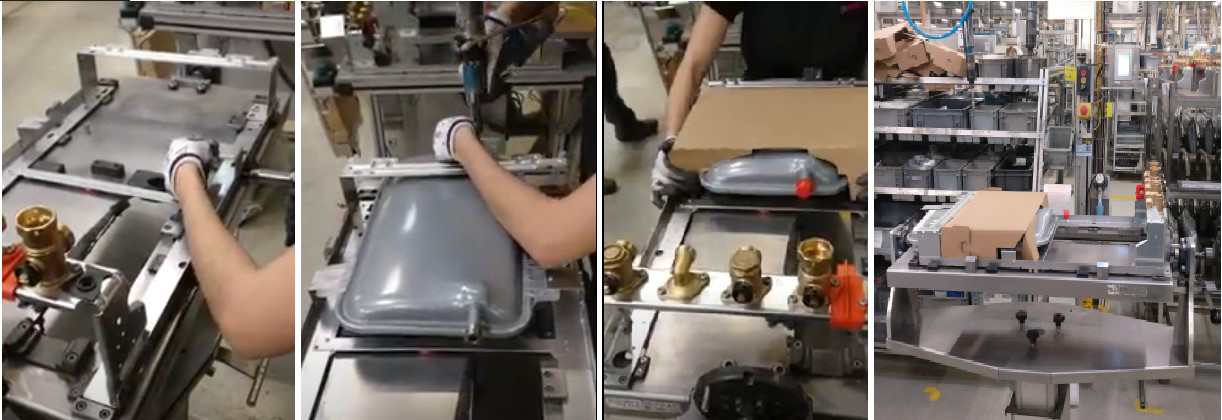
\includegraphics[width=6in]{figs/usecase.png}}
\caption{Different views of the current workstation used for the manual assemblage of the structure of a gas boiler for water heating.}
\label{fig:usecase}
\end{figure}

\section{Document Structure}

The remainder of the document is organized into five chapters. Chapter \ref{chapter:state_of_the_art} contains background material about anticipation, \acl{ml} and collaborative robotics and a review of previous work on Action Anticipation in \acs{hrc} including sensors and methods. Chapter \ref{chapter:tools_review} reviews tools that can be useful in the future implementation. Chapter \ref{chapter:work_progress} describes the progress made in the first semester. Chapter \ref{chapter:planning} portrays the planning of the second semester work and illustrates its calendarization. Chapter \ref{chapter:conclusion} concludes the document by restating the objectives of the work and the plan to achieve them.

\chapter{State of the Art}
\label{chapter:state_of_the_art}

\section{Background Material}

\subsection{Anticipation in Biology}

Anticipation is a research topic in many areas, such as biology, brain studies, psychology, social sciences, artificial intelligence, and engineering. One of the most cited definitions in the last decades and across the various fields is Rosen's \cite{Rosen1985}: "An anticipatory system is a system containing a predictive model of itself and/or its environment, which allows it to change state at an instant in accord with the model's predictions pertaining to a later instant.".

In the field of biology, \textcite{Louie2010} claims that "Much, if not most, biological behavior is model-based ..." with the referred models being the "... internal predictive models of themselves and their environments ...". \textcite{Poli2010} further claims that "... given that anticipatory behavior dramatically enhances the chances of survival, evolution itself may have found how to give anticipatory capacities to organisms, or to at least some of them.". For example, we can consider an animal predicting that it will be attacked by its predator and dodging said attack to survive.

In the case of humans, \textcite{Louie2010} also stated, "We typically decide what to do now in terms of what we perceive will be the consequences of our action at some later time." alluding to our anticipatory behavior. Therefore, human actions can result from reactive behavior when they are based on the past, from anticipatory behavior when they are based on predictions of the future, or from a mix of both.

In particular, sports is a field where, according to \textcite{Smith2016}, "Proficiency in action anticipation is relevant in many performance contexts such as anticipating the direction of a shot (in soccer, hockey, tennis, volleyball, badminton, etc.), the deceptive movement of an opponent (in soccer, basketball, rugby, football, boxing, etc.), or the movement of a partner (in figure skating, dancing, etc.).".

\subsection{Machine Learning}

Machine Learning algorithms have been increasingly more common in the last years due to, for example, their ability to deal with multidimensional data. These algorithms can automatically learn from data and make predictions or decisions, which makes them a prime candidate to use in the context of human action anticipation in collaborative environments. The most common strategies in this field are Supervised Learning, Unsupervised Learning, and Reinforcement Learning. \if{0}As we can see in Fig.~\ref{machinelearning} obtained from a review article about HRC in general, supervised learning and reinforcement learning are dominant in this area, with composite solutions surpassing unsupervised learning in the most recent year showed.

\begin{figure}[H]
\centerline{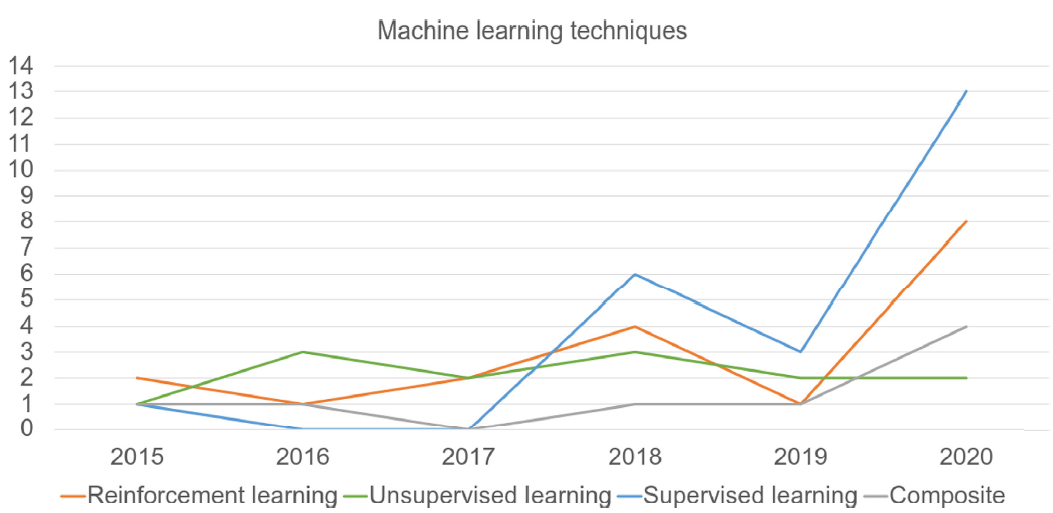
\includegraphics[width=6in]{figs/machinelearning.PNG}}
\caption{Number of articles relevant to the HRC review from each machine learning technique throughout the years\cite{Semeraro2023}}
\label{machinelearning}
\end{figure}
\fi

\subsubsection{Supervised Learning}

In Supervised Learning, the models are trained using a dataset of labeled data. The models from this group are further divided into classification, where the new instance is assigned a particular class, and Regression, where it is given a certain real number. These models must generalize the knowledge from the examples to deal with a new instance correctly that they have never seen before. Among these models, convolutional and recurrent neural networks are at the forefront of the algorithms to explore.

A Recurrent Neural Network (RNN) is a type of neural network where the output of each time step is fed back into the input at the next time step, allowing the network to remember and incorporate information from previous time steps into its processing of current and future data. This characteristic makes RNNs particularly well-suited to processing sequential data, such as text, speech, or time series data which require context or temporal dependencies. In particular, LSTM is an RNN with a more complex architecture that gives it an improved ability to backpropagate the error, making it better to train a model that classifies sequences with several time steps.

A Convolutional Neural Network (CNN) is a type of neural network made up of several convolutional layers which apply a sliding filter over the input reducing its dimension and obtaining its features. Typically, these layers are followed by one or more fully connected layers that perform the prediction using the mentioned features. This architecture makes CNNs an excellent choice to deal with data in a matrix structure such as an image because this input is too massive for manual feature engineering.

\subsubsection{Unsupervised Learning}

In Unsupervised Learning, the datasets involved have no labels; therefore, the algorithms aim to find patterns and relationships in the data. This makes them valuable for finding structure in the data, creating clusters based on common characteristics, or identifying anomalies and outliers.

\subsubsection{Reinforcement Learning}

In Reinforcement Learning, the model is trained to decide which action to take in a specific environment to maximize a particular reward function. These algorithms learn through trial and error using the reward they obtain in each iteration to improve their performance continuously. This type of learning has a certain resemblance to how humans gain knowledge, and it is useful when there is a need for an agent to make decisions in an environment that has considerable complexity, such as controlling a robot or playing a game.

\subsubsection{Transfer Learning}

Transfer Learning is a machine learning technique that uses a trained external model. Depending on the goal of its use, these models can be entirely or partially used; optionally, they can also be trained partially or fully. A common use case for this technique is when a small dataset of images is used to obtain a classifier, and a standard model cannot generalize from that reduced amount of data. In this case, a model such as VGG-16 and ResNet-50 can be used partially to extract the features with one or more fully connected layers in the end, to perform the desired classification from those features.

\subsection{Collaborative Robotics}
\label{subsection:collaborative_robotics}

Human-Robot Collaboration (HRC) consists of robots and humans working in the same workspace towards a common goal. Classical industrial robots are usually automated to perform repetitive tasks that require high physical strength. On the other hand, tasks that require cognitive knowledge, flexibility, and precision are better suited for humans, even if they are physically weaker. HRC aims to take advantage of both of their strengths and complement each others' weaknesses to increase manufacturing efficiency.

\subsubsection{Collaborative Robots}

In a Human-Robot Collaboration scenario, robots need to be different from the traditional ones, given that they will work in the same workspace as humans. According to \textcite{Castro2021}, "Collaborative robots need to be endowed with a set of abilities that enable them to act in close contact with humans, such as sensing, reasoning, and learning. In turn, the human must be placed at the centre of a careful design where safety aspects and intuitive physical interaction need to be addressed as well.". In \cite{CobotsWW}, it is stated that nowadays, collaborative robots are developed with significant advantages when working with people. For once, they have sensitive sensors that can detect the human interrupting them, causing them to stop their actions, granting more safety to the worker. They are also smaller, compact, and easy to program, among other advantages.

\subsubsection{Human-Robot Communication}

In Fig.~\ref{interaction}, we can see a diagram containing multiple data sources that can be used to implement communication between the robot and the human, along with its advantages and disadvantages.

\begin{figure}[H]
\centerline{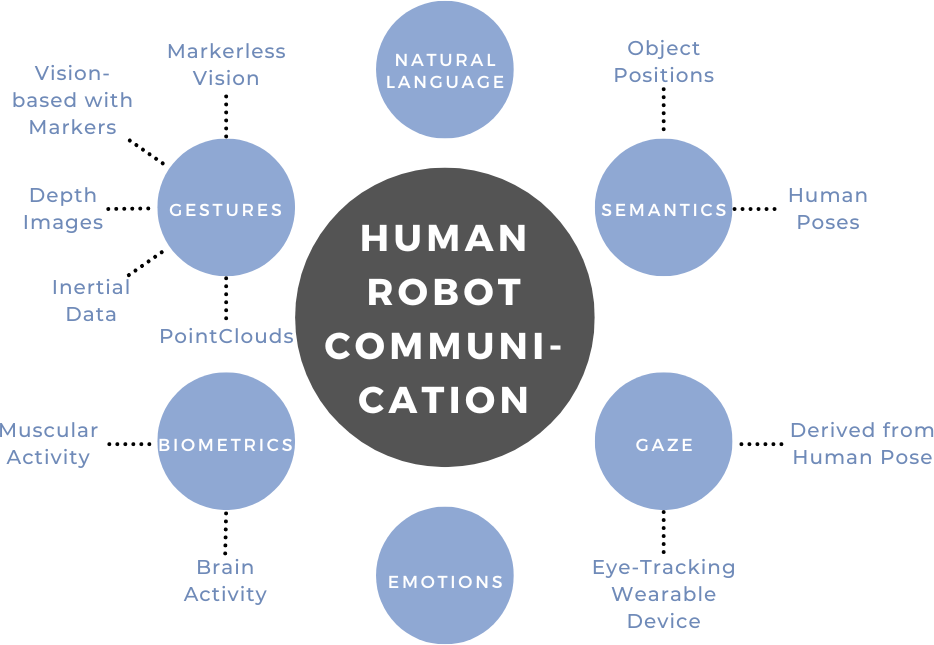
\includegraphics[width=6in]{figs/interaction.PNG}}
\caption{Advantages and Disadvantages of some Data Sources in Human-Robot Collaboration \cite{Mukherjee2022}}
\label{interaction}
\end{figure}

\begin{itemize}
\item Gestures: these are one of the main ways humans communicate, whether through simple movements or formal sign language. In work about Human-Robot Collaboration, gestures can also commonly be found since it has the advantage of resisting ambient noise. Usually, gestures are captured with vision-based methods with either an RGB or RGB-D camera, so there is no need for unnatural movements. With vision, it is possible to include markers, but these may lead to occlusions and hinder the worker's movements. Consequently, there is also work in the literature that uses markerless vision to allow more unrestricted movements. Another way to capture the movements of the human worker would be to use wearable inertial sensors, which contain accelerometers and gyroscopes, but, once again, wearables can hinder the worker's movements.

\item Natural Language: this is the most intuitive way for humans to communicate with each other. The advances in natural language processing make this a possible communication solution with robots. However, despite being intuitive, simple, effective, and even robust against lighting variations, when it comes to an industrial setting that contains significant sound noise, it becomes less valuable than the alternatives.

\item Gaze: this can be used to determine where the user's attention resides, which gives a considerable amount of information that can be used to trigger some action. There are two options to obtain the user's gaze. Wearable sensors can provide better results but are expensive and intrusive. On the other hand, algorithms that detect head pose and assume the gaze from it can also be used, which is a cheaper and non-intrusive solution.

\item Emotions: although this is a relatively new idea, some applications analyze the user's emotions from his facial expressions to have even more information in the algorithms.

\item Semantics: semantic information about the objects can also help the global workflow. For example, suppose the robot is trained to recognize certain features in objects related to how it can pick them up. In this case, the robot can pick up a new object it has never seen before if it has a similar structure. Human actions can also be represented semantically by obtaining the poses of the human as a specific set of limbs, even if only partially. During action recognition, this can be used to know which objects the worker can interact with. Having semantic information about the pose of the human body also helps in the path-planning phase of the robot since it can use this information to avoid the worker and prevent collisions.
\end{itemize}

\subsubsection{Safety}

Safety is one of the most critical topics in collaborative robotics and the first step towards establishing a human-robot collaboration environment. To ensure this, some norms were implemented: ISO 10218-1 and 10218-2. From these two standards, \textcite{Villani2018} and \textcite{Castro2021} describe the four criteria from which at least one must be met as:

\begin{enumerate}
  \item Safety-rated monitored stop: when a human enters the cobot's workspace, it completely stops;
  \item Hand guiding: when an operator manually moves the cobot, it is compliant;
  \item Speed and separation monitoring: as the human moves closer to the cobot, it becomes gradually slower;
  \item Power and force limiting: the cobot has its operation restricted in terms of force and torque.
\end{enumerate}

\begin{figure}[H]
\centerline{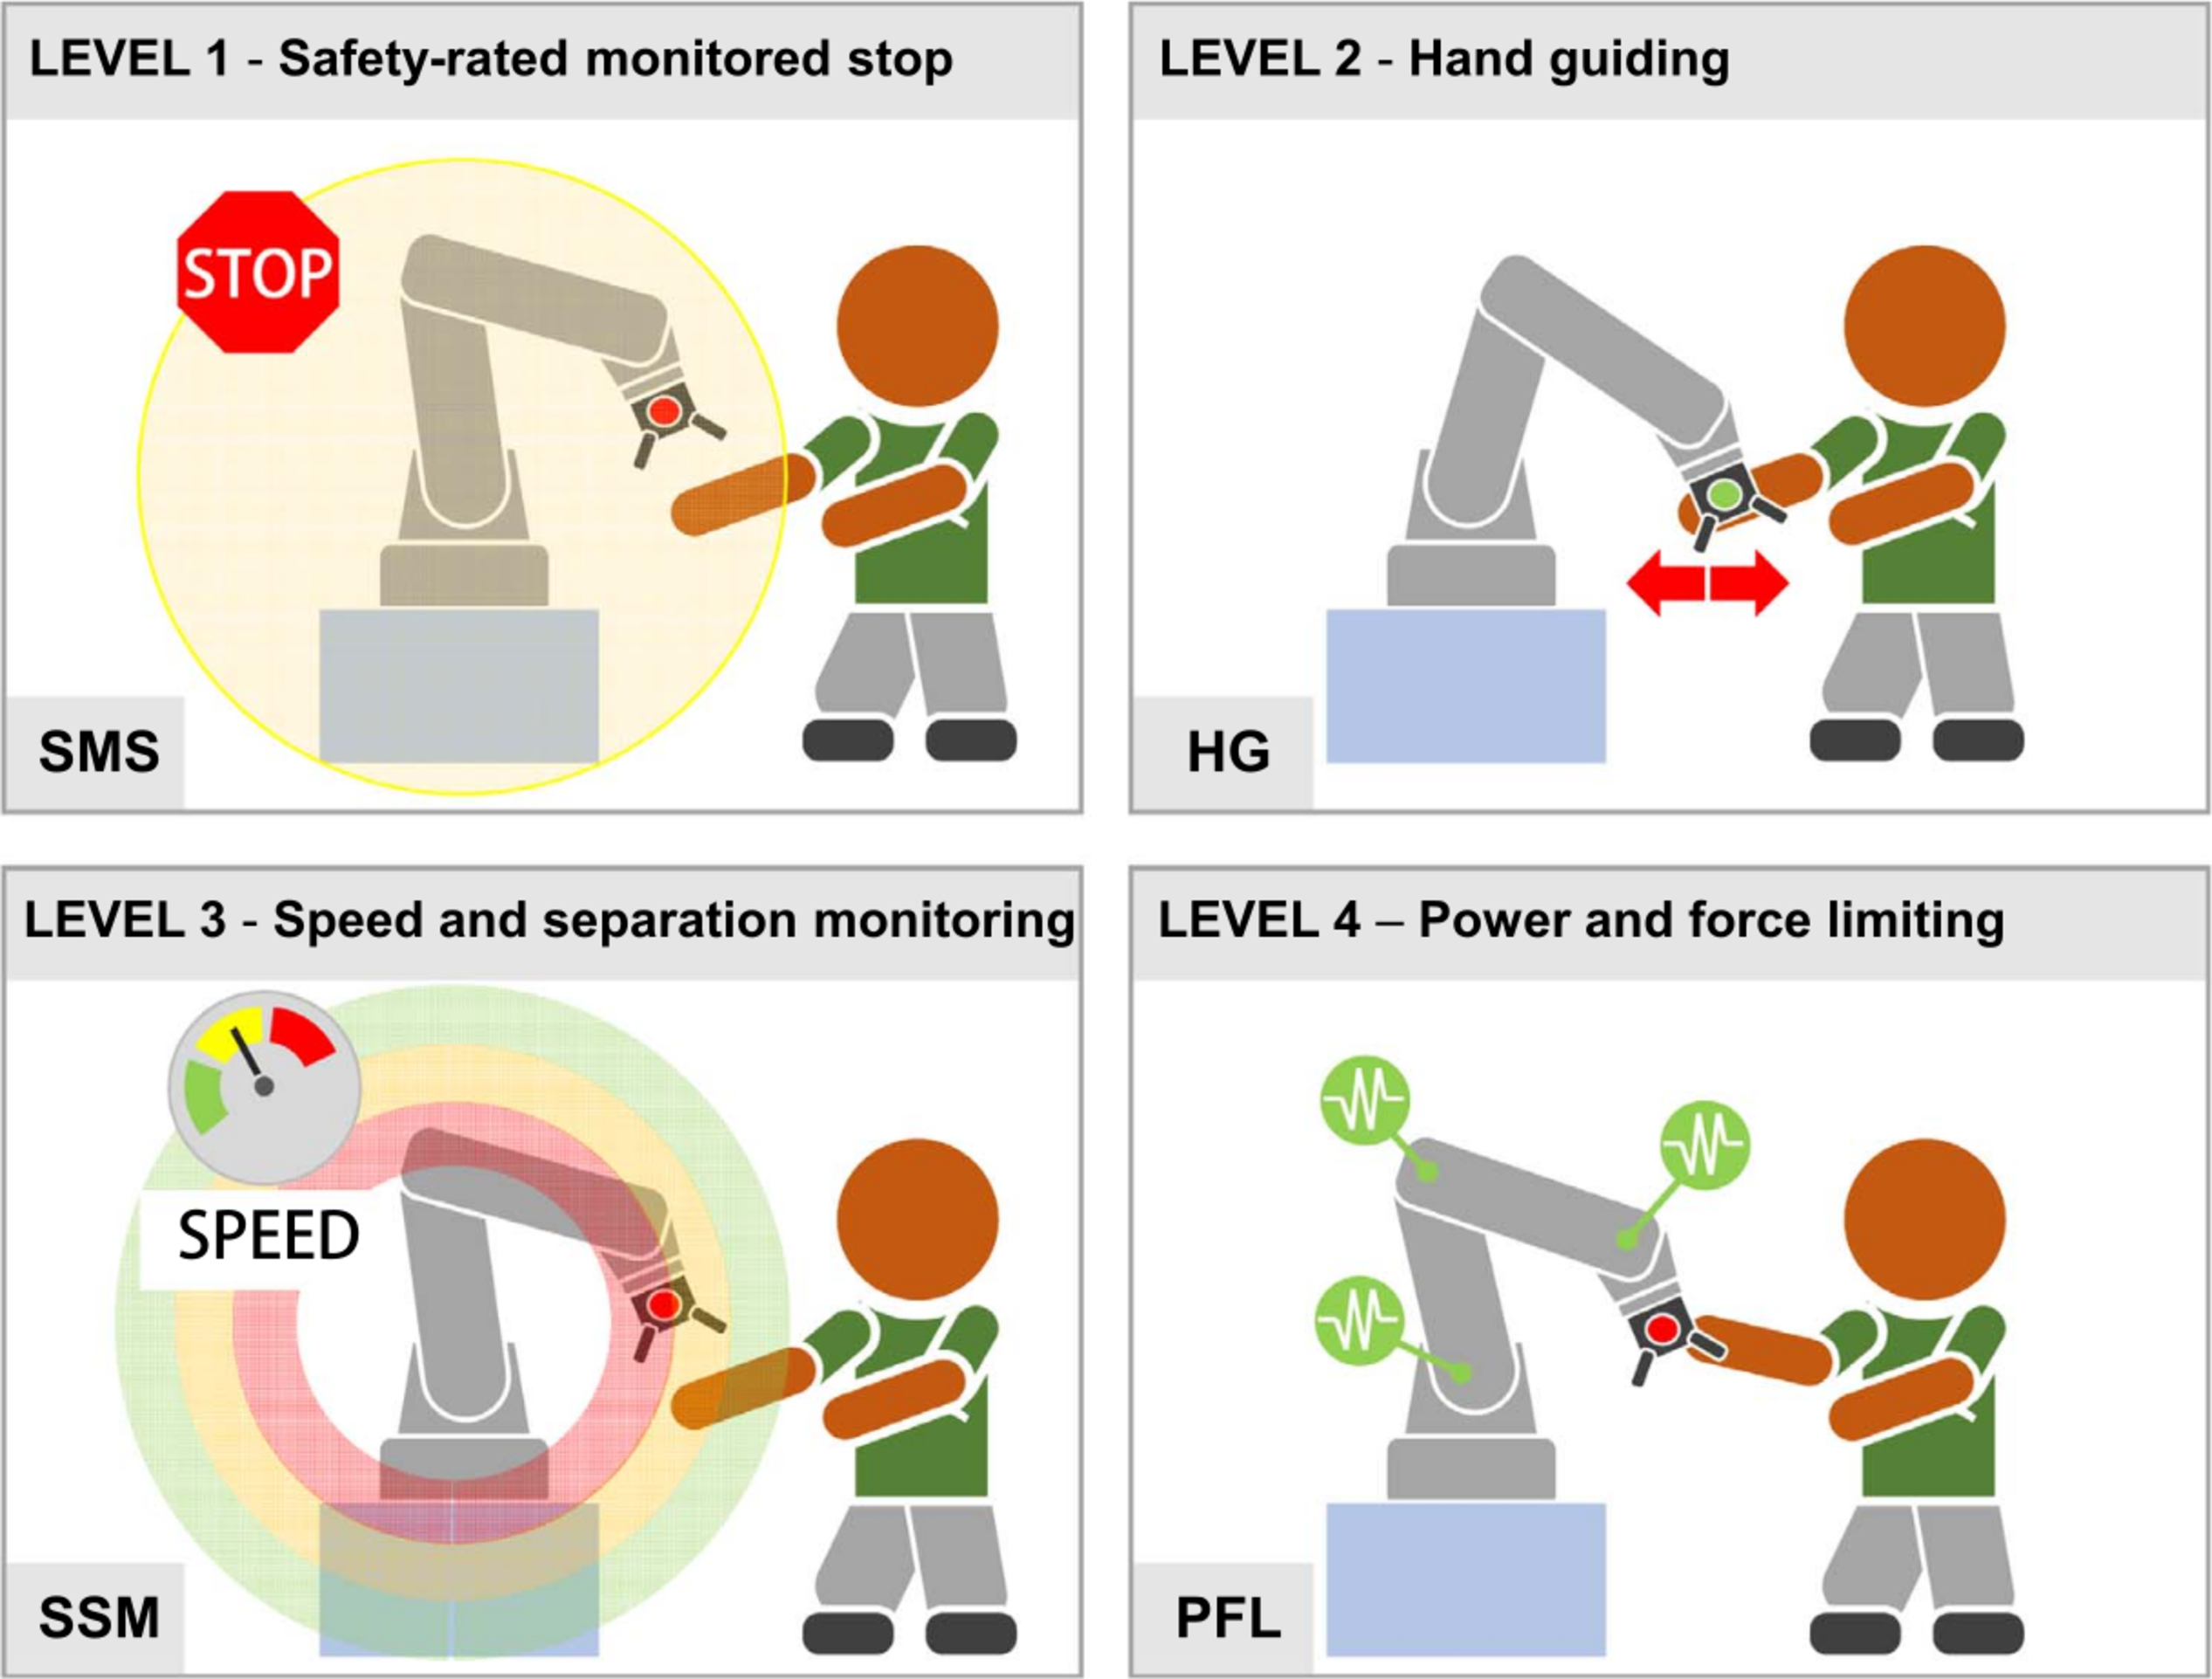
\includegraphics[width=4.5in]{figs/iso.png}}
\caption{The four collaborative operative modes identified by robot safety standards ISO modes 10218-1/2 \cite{Villani2018}}
\label{iso}
\end{figure}

\section{Data Sources and Sensors}

The first step to anticipating the following action is to know what kind of data we should collect with the sensors. Previously, several forms of communication between humans and robots were described. Still, these work in a more active way, and not all of them can be applied to action anticipation, where the user should not need to do anything for the robot to act. Essentially, there is a need to capture the human's body language.

As humans usually anticipate each other by poses and gestures, these factors became some of the most common data to perform action anticipation. Regarding sensors, most of the literature suggests using an RGB camera. Still, some works, such as the one described in \cite{Moutinho2023}, indicate the use of an RGB-D camera to capture both the color and the depth images. If wearable sensors are an option, inertial sensors also become an alternative.

In \cite{Maeda2016}, the authors also used markers to obtain the gestures of the human.

In \cite{Gammulle2019, Wu2021, Rodriguez2019, Furnari2021}, the authors went a step further and used the images but also processed the optical flow between them and used it in their algorithms.

In \cite{Canuto2021}, the authors used OpenPose (explored in detail in section \ref{section:openpose}), which is a framework with pre-trained models that receive an image, process it, and return 3D points representing the skeleton joints of the person in the image, as we can see in Fig.~\ref{openpose}.

\begin{figure}[H]
\centerline{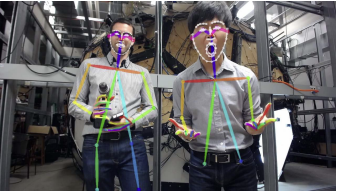
\includegraphics[width=4.5in]{figs/openpose.PNG}}
\caption{OpenPose Example\cite{Cao2021}}
\label{openpose}
\end{figure}

Humans also tend to anticipate each other by considering the other's gaze, which usually indicates his center of attention. As this is also an involuntary aspect, there is some work where gaze provides additional information, such as in \cite{Schydlo2018}, where the dataset contained the gaze of the user captured with wearable sensors, or in \cite{Canuto2021}, where the gaze was assumed from the results of an algorithm to detect the head pose.

In addition to the data related to the human, the objects present in the environment can also give valuable information about the human's following action, as is the case in \cite{Furnari2021}.

\section{Methods}

After knowing which is usually captured and provided to an algorithm, this section explores possible algorithmic solutions present in previous work.

\subsubsection{Supervised Learning}

The aim of this thesis can be represented as a Classification problem since it is possible to use a sequence of images that must be classified as a particular future action class. Using Fig.~\ref{superviseddiagram} as an example, the high-five action should be predicted before the frames that contain it are captured. The previous work with this kind of algorithm mainly includes convolutional and recurrent neural networks, with the latter being the most common.

\begin{figure}[H]
\centerline{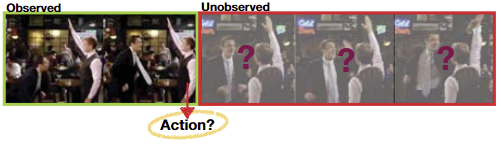
\includegraphics[width=6in]{figs/superviseddiagram.PNG}}
\caption{Action Anticipation using Supervised Learning diagram\cite{Gammulle2019}}
\label{superviseddiagram}
\end{figure}

% LSTM only examples
In \cite{Canuto2021}, the authors aimed to predict the following action using a Long Short-Term Memory (LSTM) neural network, one of the most common RNNs. In their work, they used a dataset captured with an RGB camera. From these images, they obtained the objects in the environment, the human skeleton joints extracted over time using OpenPose, and the gaze derived from the joints. Then the three data sources were given to the LSTM as input to perform the desired classification. In this process, the authors use an adaptive threshold on the uncertainty of the recurrent neural network, which makes the model need a certain level of certainty to classify the action as a particular class. This creates a more robust solution since a standard supervised learning algorithm would predict the class with the highest probability even if the model has low certainty about every category.

In \cite{Furnari2021}, the authors aimed to predict the subsequent actions that someone wearing a camera would perform and the objects he would interact with. They used three datasets containing RBG frames from which they derived the optical flow and the things in the environment. This data is then passed on to a Rolling-Unrolling LSTM. The Rolling LSTM (R-LSTM) is a network that continuously encodes the received observations and keeps an updated summary of the past. When it is time to make predictions about future actions, the Unrolling LSTM (U-LSTM) is used with its hidden and cell states equal to the current ones of the R-LSTM.

In \cite{Schydlo2018}, the authors used an encoder-decoder recurrent neural network topology to predict human actions and intent where the encoder and the decoder are both LSTM cells. At each step, the decoder returns a discrete distribution of the possible actions making this algorithm able to consider multiple action sequences, which are then subject to a pruning method that reduces them to obtain the right action finally. In their work, these algorithms were tested in two different datasets, one containing RGB images with optical markers and gaze information from wearable sensors and another with RGB-D images.

% LSTM + CNN
In \cite{Zhang2022}, the authors aimed to predict the intention of the human worker to provide him with the required piece. To achieve this, they used an RGB camera to capture the data from the environment. Then the images are given to a convLSTM framework where the CNN part is in charge of extracting features from the input images, and these features are then passed on to the LSTM to predict the intention. Additionally, another CNN is in charge of recognizing the required piece when the robot is fetching it. This article also tackles the issue of having several possible assembly orders. It solves it by creating a phase at the beginning of the collaboration in which the robot learns the assembly actions and their order from a demonstration.

% ResNet-34 + LSTM
In \cite{Moutinho2023}, the authors aimed to increase the natural collaboration between the robot and the human in an assembly station by interpreting implicit communication cues. The data related to the environment was captured using an RGB-D camera. This data was then passed on to a ResNet-34, a pre-trained neural network that extracted the features from the images. These features are used as the input to an LSTM to perform human action recognition.

% ResNet-50 + LSTM
In \cite{Gammulle2019}, the authors aimed to predict future frames while at the same time predicting the following action. In their implementation, they used public datasets with videos from which they obtained RGB images and optical flow streams. To consider both data sources, they also used two ResNet-50's, which are pre-trained networks, one to get the input features from the image and another from the optical flow, and 2 LSTMs to take into account both sequences of inputs. Then the two results are merged into a final classification. They also used two Generative Adversarial Networks (GAN) to generate the subsequent frames, but this is different from the focus of the analysis.

%% VGG-16 + TTM
In \cite{Wang2021}, the authors used video datasets to train a model that would predict a future action from the observed frames. They used three pre-trained neural networks in their work: VGG-16, TS, and ConvNet, to extract features from the images. Then these features were aggregated using a Temporal Transformer module (TTM), and finally, a progressive prediction module (PPM) would anticipate the worker's future action. This article also addresses the issue of specifying what the algorithm should consider as an action. Although most of the literature often implies that the last frames captured by the camera are considered an action, given that those are the frames that contain the last action made by the user, the authors of this article go into greater detail. They tested and evaluated how many frames should be considered as the last action to obtain the best results using a metric from \cite{Geest2016} named per-frame calibrated average precision (cAP) calculated with \eqref{eq}. In \cite{Wang2021} it is defined with

\begin{equation}
cAP=\frac{\sum_k cPrec(k) * I(k)}{P},
\label{eq}
\end{equation}

"... where  calibrated  precision $cPrec=\frac{TP}{TP+FP/w}$, $I(k)$ is an indicator function that is equal to 1 if the cut-off frame k is a true positive, $P$ denotes the total number of true positives, and $w$ is the ratio between negative and positive frames. The mean cAP over all classes is reported for final performance.".

%% CNN
In \cite{Rodriguez2019}, the authors aimed to predict the following action by first predicting the following motion images. They used datasets containing videos and then processed them to obtain motion images. These motion images become the input of a convolutional autoencoder network that generates the following motion images. These images are then passed to a Convolutional Neural Network (CNN) that processes them and makes action predictions for the future. The final action prediction is obtained from the results of the previous network and those of a second CNN, which analyzes the original RGB images.

%% architecture with TSN
In \cite{Wu2021}, the author's goal was to predict the following action someone wearing a camera would perform after some time. Initially, the optical flow was obtained from the captured images, and both were used as input to the model. The model is comprised of a Temporal Segment Networks (TSN), a CNN, and an LSTM to predict the future frame features and then use them to perform the required classification.

% Look-up table
Apart from deep learning, there are also more classical approaches such as \cite{Maeda2016}, where the authors aimed to reduce the delay in the robot's response by predicting the human worker and providing a screw or a plate accordingly. They captured the environment using an RGB camera and tracked the hand using optical markers. Then they predicted the following human action using a look-up table containing different orders for assembly actions. With the nearest neighbor algorithm, the actions of the human would be matched with a particular order. If the robot eventually notices that it did the wrong action, it would then follow a hard-coded contingency trajectory to return to the pre-grasping position. The limitation of this method is that all possible sequences need to be on the table because if they are not there, then the robot will match with a different order which may be undesirable.

\if{0}
{\color{red}
\subsection{Unsupervised Learning Solutions(possibly to delete)}

In \cite{Kato2018}, the authors attempted to recognize human actions using the trajectories of skeleton joints. The environment was captured using a RGB camera and then the joints were obtained using OpenPose.
}

{\color{red} explain the rest of the model} 
\fi

\subsubsection{Reinforcement Learning}

% POMDP
In \cite{Gorur2018}, the authors aimed to make the human-robot interaction more natural by detecting unexpected conditions where the human will not need the robot's assistance, such as when the human's current intention is unknown or irrelevant to the robot or when even though the human's intent is relevant, that task is done only by the human. They used the algorithm Partially Observable Markov Decision Process (POMDP) to achieve this. The training was done with simulation with the model learning a policy by having a positive reward if the task was accomplished and a negative reward if the robot tried to help the human in a situation where it should not.

{\color{red} I am planning to add more examples of reinforcement learning}

\section{Human-Robot Collaboration Safety}

Finally, safety is a topic that must always be mentioned when robots work with humans, especially in human-robot collaboration. Although this topic was also covered in subsection \ref{subsection:collaborative_robotics}, many articles in action anticipation also explore their strategies to ensure the worker's safety.

In \cite{Zhang2022}, the authors defined speed limits on the robot and ensured that the robot would avoid the workspace of the human. Then when it needs to move closer to the user, its speed is reduced to guarantee the user's safety.

In \cite{Wu2023}, the authors used deep deterministic policy gradient (DDPG) to plan the robot's trajectory so that the robot would not collide with the human to guarantee his safety.

In \cite{Psarakis2022}, the authors attempted to create a sense of anticipation in humans towards the robot's movements through visual cues of the robot's upcoming action, which is the reverse of what it is being tried to achieve in the other reviewed papers. As with the previous article, they also made it so the robot must reduce its movement speed when close to the robot. Although it was only tested in the Virtual Reality simulation shown in Fig.~\ref{vr}, where the users feel safer, they concluded that the efficiency of the collaboration was increased, and the user had a greater feeling of safety and trust. Furthermore, knowing what the robot will do next also decreases the risk of a collision since the user will avoid the space where the robot is working, increasing safety.

\begin{figure}[H]
\centerline{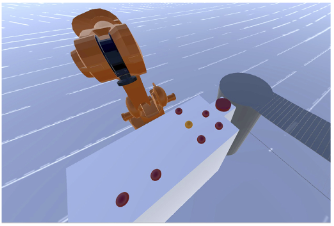
\includegraphics[width=3.5in]{figs/reverse.PNG}}
\caption{VR Simulation of \cite{Psarakis2022}, the orange means the robot will pick that puck next}
\label{vr}
\end{figure}

In \cite{Mukherjee2022}, it is also stated that limiting the power and force of the robot decreases the gravity of the consequences of a possible collision, increasing safety.
\chapter{State of the Art}
\label{chapter:state_of_the_art}

\section{Tools Review}

\subsubsection{ROS}

\subsubsection{Tensorflow}

\subsubsection{The Robot}

\section{Background Material}

{\color{gray}
(ideas) relevant and established knowledge assumed as known
}

\section{Previous Work}

\subsection{Data Sources and Sensors}

In \cite{Schydlo2018} part of the data contained information about the gaze of the user from wearable sensors.

In \cite{Furnari2021} the authors detected the motion using the optical flow obtained from the RGB images and from the object related features using a object detector.

In \cite{Gammulle2019}, \cite{Wu2021} and \cite{Rodriguez2019} the authors used both the images and the optical flow obtained from them.

In \cite{Moutinho2023} the authors used a RGB-D camera so as to capture depth.

\subsection{Algorithms}

Machine Learning algorithms have been increasingly more common in the context of action anticipation in collaborative environments. These are divided in 3 groups: Supervised Learning, Unsupervised Learning and Reinforcement Learning.

\subsubsection{Supervised Learning}

In \cite{Maeda2016} the authors predicted the next human action using a look-up table containing different orders for assembly actions and with the nearest neighbor algorithm the actions of the human would be matched with a certain order.

In \cite{Canuto2021} the authors used a Long Short-Term Memory (LSTM) Neural Network to handle classifying the next action using the human skeleton joints of several frames over time. These joints were obtained using OpenPose on the captured images.

In \cite{Schydlo2018} the authors used a encoder-decoder recurrent neural network topology to predict human actions and intent.

In \cite{Zhang2022} the authors use ConvLSTM to predict the intention of the user.

In \cite{Furnari2021} the authors use a Rolling-Unrolling LSTM. {\color{red} (transcribed) "A Rolling” LSTM (RLSTM) continuously encodes streaming observations and keeps an updated summary of what has been observed so far. When an anticipation is required, the “Unrolling” LSTM (U-LSTM) is initialized with the current hidden and cell states of the R-LSTM (which encode the summary of the past) and makes predictions about the future".}

In \cite{Gammulle2019} the authors used 2 ResNet50's {\color{red} (put reference here)} to obtain the input features and 2 LSTM's to take into account the sequence of inputs. Then the 2 results are merged into a final classification.

In \cite{Wu2021} the authors used Temporal Segment Networks (TSN) to predict the future action.

In \cite{Wang2021} the authors used VGG-16, TS, ConvNet to extract features from the images, then these features are aggregated using a Temporal Transformer module (TTM) and finally, a progressive prediction module (PPM) will anticipate the future action.

In \cite{Rodriguez2019} the authors processed the images to obtain motion images and then used a convolutional autoencoder network to generate the next motion images. These images are then passed to a Convolutional Neural Network (CNN) that processes them and makes action predictions for the future. The result of this network and another CNN which analyzes the static images results in the final action prediction.

In \cite{Gorur2018} the authors partially observable Markov decision process (POMDP) to handle unexpected conditions such as when the human’s current intention is unknown or irrelevant to the robot or when even though the human’s intention is relevant, the human does not need the robot’s assistance.

In \cite{Moutinho2023} the authors used convolutional neural network with 34 layers and a long-short term memory recurrent neural network (ResNet-34 + LSTM) obtaining assembly context through action recognition of the tasks performed by the operator.

\subsubsection{Unsupervised Learning}

\subsubsection{Reinforcement Learning}

\subsection{Definition and Order of Actions}

In general, the last frames captured by the camera are considered an action in the literature of this theme.

In \cite{Wang2021} the authors tested how much frames should be considered as the last action in order to obtain the best results. These tests are evaluated using a metric from {\color{red} (put reference here)} named per-frame calibrated average precision (cAP).

In \cite{Maeda2016} the authors used a look-up table containing different orders for assembly actions and with the nearest neighbor algorithm the actions of the human would be matched with a certain order. The limitation of this method is that all of the possible sequences need to be on the table because if they are not there then the robot will match with a different order which may be undesirable.

In \cite{Canuto2021} the authors use an adaptive threshold on the uncertainty of the recurrent neural network which makes it so the model needs to a certain level of certainty in order to classify the action as a certain class.

In \cite{Schydlo2018} the authors predicted multiple possible actions while the model was unsure of what would be the next action.

In \cite{Zhang2022} the authors made it so there would be a phase when the robot learned from demonstration which were the assembly actions and its order.

\subsection{Human-Robot Collaboration Safety}

In \cite{Zhang2022} the authors defined speed limits on the robot and made it so the robot avoids the workspace of the human. Then when it needs to move closer to the user, its speed is reduced in order to guarantee the safety of the user.

In \cite{Psarakis2022} the authors attempted to create a sense of anticipation in humans towards the robot's movements through visual cues of the robot's upcoming action. As with the previous article, they also make it so the robot reduces its motion speed when close to the robot. Although it was only tested in VR where the users feels safer, they concluded that the efficiency of the collaboration was increased and knowing what the robot will do next also increases safety.
\chapter{Work Progress}
\label{chapter:work_progress}

{\color{gray}
(ideas) Progress done until the end of the semester
}



% End of Thesis text ---------------------------------------------------------
% Including files is advised:


%Appendix

\backmatter
\nocite{*}

%Print all used references

\begingroup
\renewcommand{\bibfont}{\footnotesize}

%Redefine References name
\defbibheading{bibliography}[References]{
	\chapter{#1}
}
\SingleSpacing
\setlength\bibitemsep{8pt}
\printbibliography[heading=bibliography]
\endgroup


%Load appendix
%\include{appendix-a}


\end{document}
